\chapter{Tecnologie e principi teorici}
\label{cap:tecnologie-principi-teorici}

\intro{Il capitolo presenta il quadro teorico e tecnologico di riferimento del progetto, descrivendo i principali approcci e strumenti per il monitoraggio delle prestazioni applicative. Vengono illustrate le tecnologie analizzate e le motivazioni che hanno guidato la scelta della soluzione, in relazione ai requisiti e agli obiettivi del sistema di osservabilità sviluppato.}\\

\section{APM e Observability}
\label{sec:apm-observability}
L'osservabilità di un sistema si basa sull'analisi congiunta di tre pilastri fondamentali: metriche, log e tracce. 
\begin{itemize}
    \item \textbf{Logs}: un log è un record testuale di un evento ad un orario specifico, come un tentativo di accesso, un errore di sistema o una transazione completata. I log forniscono dettagli di contesto che aiutano a diagnosticare problemi specifici;
    \item \textbf{Metriche}: una metrica è una misurazione numerica di un aspetto specifico delle prestazioni del sistema, come l'utilizzo della \gls{cpug}, la latenza delle richieste o il numero di utenti attivi;
    \item \textbf{Tracce}: una traccia rappresenta il percorso di una singola richiesta attraverso i vari componenti di un sistema distribuito, consentendo di visualizzare il flusso delle operazioni e identificare i colli di bottiglia.
\end{itemize}
Un sistema \gls{apmg} moderno integra questi aspetti per fornire una visione completa dello stato e del comportamento applicativo. Nel contesto del monitoraggio di applicazioni \emph{web} come \emph{PetClinic}, l'osservabilità consente di analizzare i dati di performance raccolti dal sistema di \gls{apmg} per identificare e risolvere problemi, ottimizzare le prestazioni e migliorare l'esperienza utente complessiva.


\section{Approcci e tecnologie per il monitoraggio}
\label{sec:approcci-tecnologie-monitoraggio}
Nel mondo dell'\emph{Application Performance Monitoring} esistono diversi approcci e tecnologie per raccogliere, analizzare e visualizzare i dati di telemetria. \\
Il monitoraggio delle prestazioni può essere realizzato mediante diverse strategie, che si distinguono per tipo di dati raccolti, modalità di raccolta e grado di integrazione con l'applicazione.


\subsection{Approcci principali}
Gli approcci al monitoraggio delle applicazioni possono essere classificati in base alla modalità di raccolta dei dati e al livello di osservabilità fornito. \\
Tra i principali si distinguono:
\begin{itemize}
\item \textbf{Monitoraggio basato sugli agenti (Agent-based monitoring):} prevede l'integrazione di componenti software, detti \emph{agent}, all'interno dell'applicazione o dell'infrastruttura. Questi raccolgono metriche, log e tracce in tempo reale, offrendo una visione complessiva del sistema. È il modello adottato da strumenti come \emph{Elastic APM}, \emph{Datadog} e \emph{New Relic};

\item \textbf{Monitoraggio senza agenti (Agentless monitoring):} in questo caso la raccolta dei dati avviene tramite l'analisi di log o metriche esposte da servizi esterni, senza modificare il codice dell'applicazione. Sebbene riduca l'invasività, questo approccio offre un livello di dettaglio inferiore rispetto ai sistemi \emph{agent-based};

\item \textbf{Distributed tracing:} metodo che consente di tracciare l'intero ciclo di vita di una richiesta distribuita tra più servizi o microservizi, associando a ciascun evento un identificativo univoco;

\item \textbf{Synthetic monitoring:} utilizza richieste simulate e test automatizzati per verificare la disponibilità e le prestazioni delle applicazioni da diverse località geografiche. È utile per individuare problemi prima che impattino sugli utenti reali dell'applicazione;

\item \textbf{Real User Monitoring (RUM):} misura le prestazioni dal punto di vista dell'utente reale, analizzando tempi di caricamento, interazioni e metriche di esperienza. Combinato con il monitoraggio sintetico, fornisce una visione completa della user experience indicata con il termine \gls{eum}\glsfirstoccur.
\end{itemize}
Nel corso del monitoraggio di \emph{PetClinic}, l'approccio adottato integra principalmente il monitoraggio basato sugli agenti, il \emph{distributed tracing} e il \emph{Real User Monitoring}, al fine di ottenere una visione dettagliata e completa delle prestazioni dell'applicazione.


\subsection{Tecnologie e piattaforme note}
Negli ultimi anni si sono affermate diverse piattaforme e \emph{framework} dedicati al monitoraggio e all'osservabilità, che adottano architetture e modelli di raccolta dati differenti. \\
Tra le più rilevanti si trovano:
\begin{itemize}
\item \textbf{Elastic Stack (ELK):} una delle soluzioni \emph{open source} più diffuse, integra \emph{Elasticsearch}, \emph{Logstash} e \emph{Kibana}, estesa con \emph{Elastic APM} per il tracciamento delle prestazioni. Offre un ecosistema unificato per metriche, log e tracce;

\item \textbf{OpenTelemetry:} standard \emph{open source} promosso dalla \emph{Cloud Native Computing Foundation (CNCF)} per la raccolta e l'esportazione di dati di telemetria. Fornisce \gls{sdk}\glsfirstoccur e agenti per numerosi linguaggi di programmazione, garantendo interoperabilità tra sistemi di osservabilità differenti;

\item \textbf{Prometheus e Grafana:} soluzione \emph{open source} focalizzata sulle metriche. \emph{Prometheus} raccoglie e memorizza dati temporali, mentre \emph{Grafana} li visualizza in \emph{dashboard} personalizzabili. È molto usata in ambienti \emph{cloud-native} e \emph{Kubernetes};

\item \textbf{Datadog, New Relic, Dynatrace:} piattaforme commerciali che offrono funzionalità avanzate di \gls{apmg}, monitoraggio dell'infrastruttura e analisi basata su \emph{machine learning}.;
\end{itemize}
Le soluzioni open source, come \emph{Elastic Stack} e \emph{OpenTelemetry}, offrono maggiore flessibilità e possibilità di personalizzazione, rendendole particolarmente adatte per ambienti di sviluppo e sperimentazione. \\
Nel contesto del progetto di monitoraggio \emph{PetClinic}, l'attenzione si è concentrata sull'integrazione tra l'\emph{Elastic Stack} e \emph{OpenTelemetry}, con l'obiettivo di realizzare una soluzione di monitoraggio estendibile e compatibile con l'infrastruttura aziendale.


\section{Tecnologie e strumenti utilizzati}
\label{sec:tecnologie-strumenti}
Di seguito viene data una panoramica delle tecnologie e degli strumenti utilizzati.

\subsection{Elastic Stack}

\subsection*{Elasticsearch}
Elasticsearch è un motore di ricerca e analisi distribuito basato su \emph{Apache Lucene}, progettato per gestire grandi volumi di dati in tempo reale. Fornisce funzionalità avanzate di ricerca \emph{full-text}, analisi dei dati e aggregazioni, rendendolo ideale per applicazioni di monitoraggio, analisi dei \emph{log} e \emph{business intelligence}. Elasticsearch supporta un'architettura scalabile e flessibile, consentendo di distribuire i dati su più nodi e cluster per garantire alta disponibilità e prestazioni elevate.
\begin{figure}[H] 
    \centering 
    
\includegraphics[width=4cm]{/logos/elasticsearch.png} 
    \caption{Figura 4.1 - Elasticsearch}
\end{figure}


\subsection*{Kibana}
Kibana è uno strumento di visualizzazione e analisi dei dati open source, progettato per lavorare in stretta integrazione con Elasticsearch. Fornisce un'interfaccia utente intuitiva che consente agli utenti di creare \emph{dashboard} interattive, visualizzare grafici, mappe e tabelle, e analizzare i dati in tempo reale. Kibana supporta una vasta gamma di visualizzazioni personalizzabili e offre funzionalità avanzate come il filtraggio dei dati, la ricerca \emph{full-text} e l'esplorazione delle relazioni tra i dati, rendendolo uno strumento potente per l'analisi dei \emph{log}, il monitoraggio delle prestazioni e la \emph{business intelligence}.
\begin{figure}[H] 
    \centering 
    
\includegraphics[width=4cm]{/logos/kibana.png} 
    \caption{Figura 4.2 - Kibana}
\end{figure}


\subsection*{Elastic Agent e Fleet}
Elastic Agent è un agente unificato sviluppato da Elastic che consente di raccogliere, monitorare e proteggere i dati da diverse fonti in modo semplice ed efficiente. Integrando funzionalità di raccolta dati, sicurezza e monitoraggio, Elastic Agent semplifica la gestione degli agenti e riduce la complessità operativa. Fleet è una funzionalità di gestione centralizzata all'interno di Kibana che consente di distribuire, configurare e monitorare gli Elastic Agent in modo scalabile e automatizzato. Attraverso Fleet, gli utenti possono gestire facilmente le policy di raccolta dati, aggiornare gli agenti e monitorare lo stato della loro infrastruttura da un'unica interfaccia.


\subsection*{OpenTelemetry}
\begin{figure}[H] 
    \centering 
    
\includegraphics[width=4cm]{/logos/OpenTelemetry.png} 
    \caption{Figura 4.3 - OpenTelemetry}
\end{figure}


\subsection*{Elastic APM e APM Server}
\begin{figure}[H] 
    \centering 
    
\includegraphics[width=4cm]{/logos/ElasticAPM.png} 
    \caption{Figura 4.4 - Elastic APM}
\end{figure}


\subsection*{RUM Agent e Synthetic Monitoring}


\subsection*{MCP}


\subsection{Linguaggi di programmazione}
\subsection*{Python}
\begin{figure}[H] 
    \centering 
    
\includegraphics[width=4cm]{/logos/Python_logonormal.png} 
    \caption{Figura 4.5 - Python}
\end{figure}


\subsection*{JavaScript}
\begin{figure}[H] 
    \centering 
    
\includegraphics[width=4cm]{/logos/javascript.png} 
    \caption{Figura 4.6 - JavaScript}
\end{figure}


\subsection*{Java}
\begin{figure}[H] 
    \centering 
    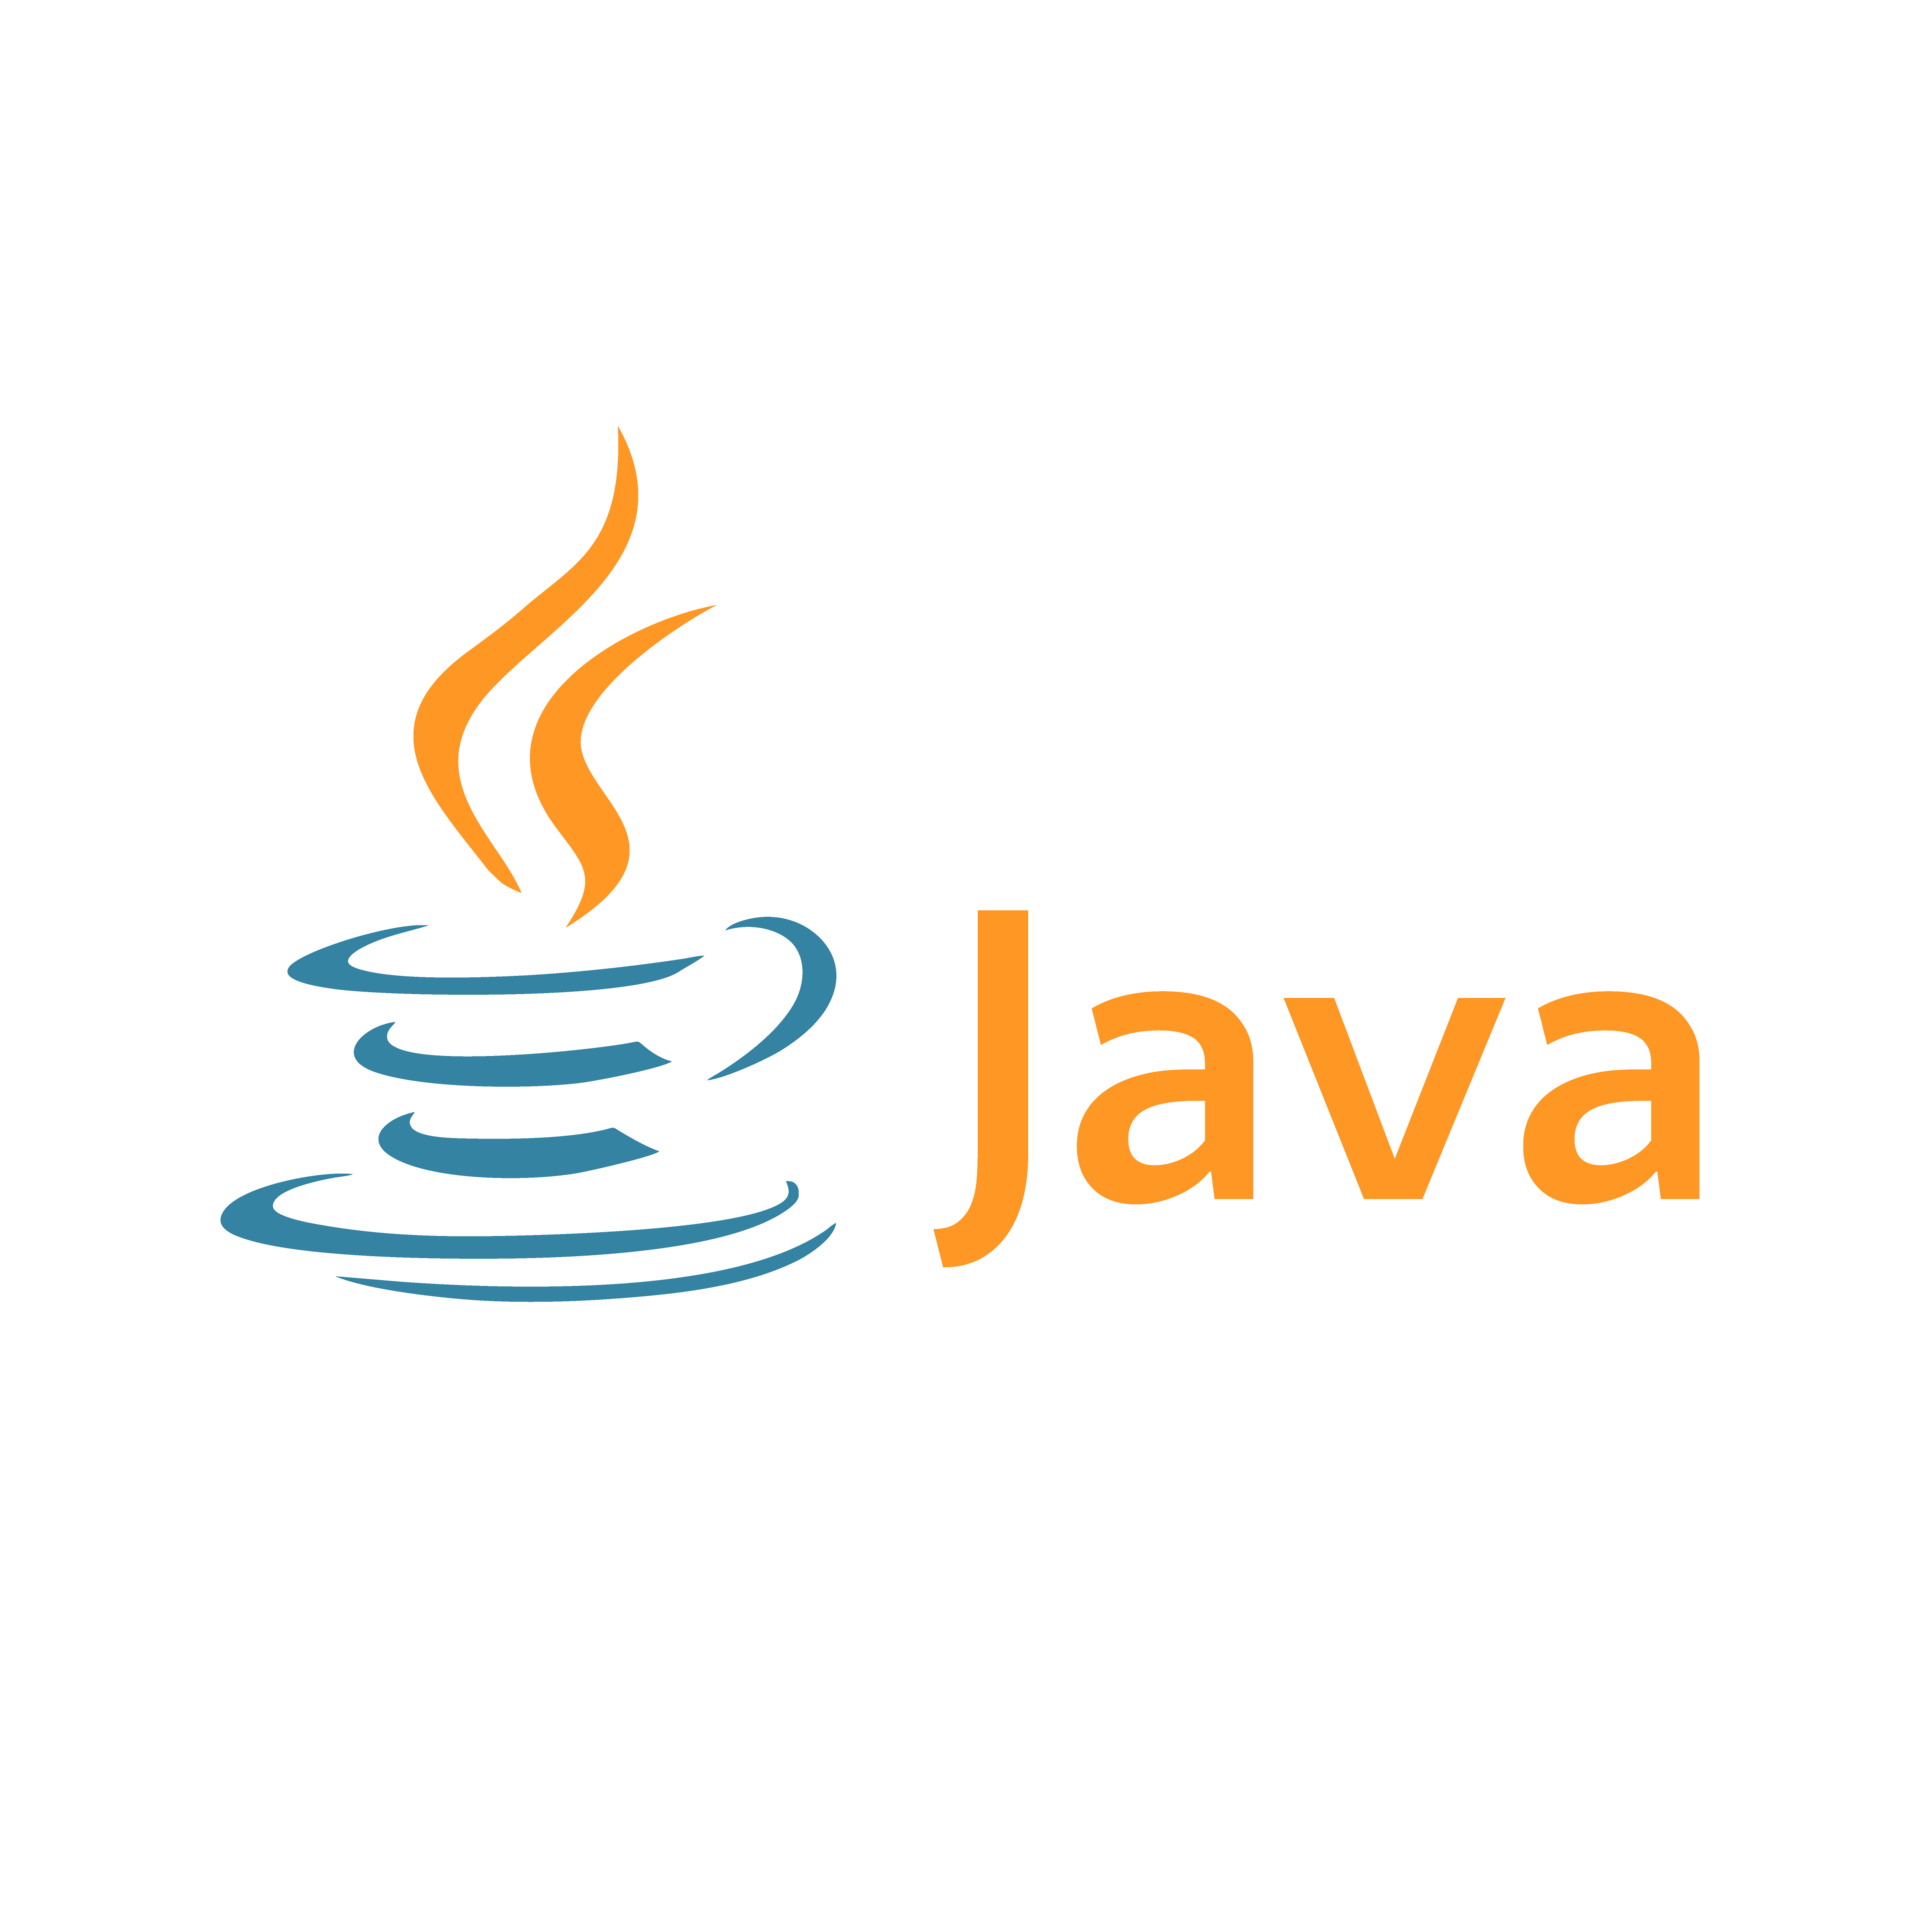
\includegraphics[width=4cm]{/logos/java.png} 
    \caption{Figura 4.7 - Java}
\end{figure}


\subsection{Framework e librerie}
\subsection*{Node.js}
\begin{figure}[H] 
    \centering 
    
\includegraphics[width=4cm]{/logos/nodeJS.png} 
    \caption{Figura 4.8 - Node.js}
\end{figure}


\subsection*{Spring Boot}
\begin{figure}[H] 
    \centering 
    
\includegraphics[width=4cm]{/logos/spring.png} 
    \caption{Figura 4.9 - Spring}
\end{figure}


\subsection*{Selenium}
\begin{figure}[H] 
    \centering 
    
\includegraphics[width=4cm]{/logos/selenium.png} 
    \caption{Figura 4.10 - Selenium}
\end{figure}


\subsection{Strumenti di sviluppo}
\subsection*{VSCode}
\begin{figure}[H] 
    \centering 
    
\includegraphics[width=4cm]{/logos/vscode.png} 
    \caption{Figura 4.11 - VSCode}
\end{figure}


\subsection{Database}
\subsection*{MySQL}
\begin{figure}[H] 
    \centering 
    
\includegraphics[width=4cm]{/logos/Mysql_barattolo.png} 
    \caption{Figura 4.12 - MySQL}
\end{figure}


\newpage
\section{Criteri di scelta della soluzione}
\label{sec:criteri-scelta-soluzione}
Le principali motivazioni che hanno guidato la scelta della soluzione di monitoraggio basata su \emph{Elastic Stack} e \emph{OpenTelemetry} sono:
\begin{itemize}
    \item \textbf{Open source e flessibilità:} entrambe le tecnologie sono open source, consentendo una maggiore personalizzazione e adattabilità alle esigenze specifiche del progetto;
    \item \textbf{Scalabilità:} la soluzione è progettata per gestire grandi volumi di dati in ambienti distribuiti, garantendo prestazioni elevate anche con l'aumento del carico di lavoro;
    \item \textbf{Ecosistema completo:} \emph{Elastic Stack} offre un ecosistema completo per la raccolta, l'analisi e la visualizzazione dei dati, semplificando la gestione del sistema di monitoraggio;
    \item \textbf{Requisiti aziendali:} la scelta è stata influenzata dalla necessità di integrare il sistema di monitoraggio con l'infrastruttura esistente dell'azienda, che già utilizza componenti dell'\emph{Elastic Stack};
    \item \textbf{Comunità attiva:} entrambe le tecnologie vantano una comunità di sviluppatori attiva e in crescita, che contribuisce al miglioramento continuo delle piattaforme e fornisce supporto agli utenti.
\end{itemize}


\section{Integrazione con l'ambiente esistente}
\label{sec:integrazione-ambiente-esistente}
L'integrazione della soluzione di monitoraggio è stata progettata tenendo conto delle specifiche dell'ambiente tecnico aziendale, basato su infrastrutture Linux e containerizzazione tramite Docker. \\
Tutti i componenti dell'\emph{Elastic Stack} sono stati distribuiti in un ambiente isolato, mantenendo la compatibilità con le versioni approvate dall'azienda. \\
La comunicazione tra l'applicazione \emph{web PetClinic} e il sistema di osservabilità avviene tramite l'agente \emph{OpenTelemetry Java}, che esporta i dati di telemetria verso l'\emph{Elastic APM Server} gestito da \emph{Fleet}. 
L'approccio adottato permette un'integrazione trasparente con l'ambiente esistente, garantendo la scalabilità del sistema e la possibilità di estendere la soluzione ad altri servizi o applicazioni monitorate nel futuro.

%\section{Ciclo di vita del software}
%\label{sec:ciclo-vita-software}

%\section{Progettazione}
%\label{sec:progettazione}

%\subsubsection{Namespace 1} %**************************
%Descrizione namespace 1.

%\begin{namespacedesc}
    %\classdesc{Classe 1}{Descrizione classe 1}
    %\classdesc{Classe 2}{Descrizione classe 2}
%\end{namespacedesc}


%\section{Design Pattern utilizzati}

%\section{Codifica}
